\documentclass[12pt]{article}
\usepackage{makeidx}
\usepackage{multirow}
\usepackage{multicol}
\usepackage[dvipsnames,svgnames,table]{xcolor}
\usepackage{graphicx}
\usepackage{epstopdf}
\usepackage{ulem}
\usepackage{hyperref}
\usepackage{amsmath}
\usepackage{amssymb}
\author{Omkar Mohite}
\title{}
\usepackage[paperwidth=595pt,paperheight=841pt,top=72pt,right=72pt,bottom=72pt,left=72pt]{geometry}

\makeatletter
	\newenvironment{indentation}[3]%
	{\par\setlength{\parindent}{#3}
	\setlength{\leftmargin}{#1}       \setlength{\rightmargin}{#2}%
	\advance\linewidth -\leftmargin       \advance\linewidth -\rightmargin%
	\advance\@totalleftmargin\leftmargin  \@setpar{{\@@par}}%
	\parshape 1\@totalleftmargin \linewidth\ignorespaces}{\par}%
\makeatother 

% new LaTeX commands


\begin{document}
\begin{center}

\textbf{{\LARGE Configuring JY-MCU Bluetooth module using AT (Attention)
commands}}
\end{center}
\begin{enumerate}
	\item \textbf{{\large About JY-MCU Bluetooth module:}}

\begin{enumerate}
	\item \textbf{Introduction:}



This is a Bluetooth Wireless module that provides a simple interface for
connecting to Arduino, AVR, Firewing, USB to serial converter and other
microcontroller applications.

The module provides a method to connect wirelessly with a PC or Bluetooth phone
to transmit/receive embedded data such as GPS data, ADC voltage reading and other
parameters.


	\item \textbf{Technical Specification:}


\begin{itemize}
	\item JY-MCU Bluetooth Wireless Serial Port Module with free extension cable designed
for easy use with Arduino boards,Atmega boards and Firewing boards.	
\item Supply voltage can be between 3.6 to 6V DC. IOs are 5V tolerant. 
	\item Bluetooth V2.0+EDR (Enhanced Data Rate) 3Mbps 
	\item Bluetooth SPP (Serial Port Protocol) 
	\item Easy to connect this module with any standard Bluetooth device, just search and key "1234" passcode. 
	\item Baud rate: 38400 bps, 9600 bps default
	\item Module requires no setup. 
	\item Dimensions: 1.73 in x 0.63 in x 0.28 in (4.4 cm x 1.6 cm x 0.7 cm) 
\end{itemize}

\textbf{    \\                     Fig 1:} JY-MCU Bluetooth module
\begin{center}
	\graphicspath{ {images/} }
	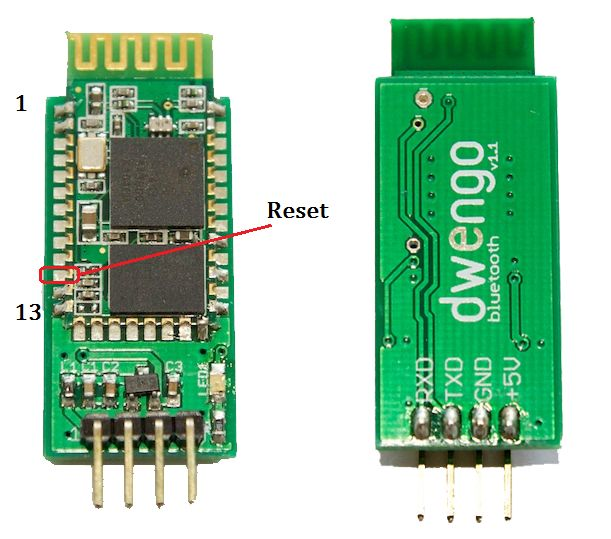
\includegraphics[width=9cm, height=9cm]{JY_MCU}
\end{center}

	\item \textbf{Application circuit:}
\begin{center}

{\raggedright

\vspace{3pt} \noindent
\begin{tabular}{|p{132pt}p{132pt}|}
\hline
\multicolumn{2}{|l|}{\parbox{264pt}{\raggedright 
\textbf{JY-MCU Bluetooth Module Pinout{\small s}}
}} \\
\parbox{132pt}{\raggedright 
\textbf{Pin No{\small .}}
} & \parbox{132pt}{\raggedright 
\textbf{Signal Description }
} \\
\parbox{132pt}{\raggedright 
{\small 1}
} & \parbox{132pt}{\raggedright 
Key (No pin)
} \\
\parbox{132pt}{\raggedright 
{\small 2}
} & \parbox{132pt}{\raggedright 
VCC +3.6v to +6v DC
} \\
\parbox{132pt}{\raggedright 
{\small 3}
} & \parbox{132pt}{\raggedright 
GND- Ground Connection
} \\
\parbox{132pt}{\raggedright 
{\small 4}
} & \parbox{132pt}{\raggedright 
TXd -Tx from module
} \\
\parbox{132pt}{\raggedright 
{\small 5}
} & \parbox{132pt}{\raggedright 
RXD- Rx for the module
} \\
\hline
\end{tabular}
\vspace{2pt}

}

\end{center}
	\item \textbf{1.4.	Pairing your Bluetooth module with your Computer/Laptop: }


\begin{itemize}
	\item Turn on your laptop Bluetooth Wireless or plug the Bluetooth USB module into your desktop PC. .
	\item Task bar will show the connected status of the blue tooth device. 
	\item Add Device by right click on the Bluetooth task bar icon. 
	\item You will find a device named “Linvor”. Choose this and complete the installation until your board blue tooth module is paired with computer Bluetooth. 
	\item Use the pass code or pin is 1234 for this connection if prompted.
\end{itemize}
\end{enumerate}

	\item \textbf{{\large AT commands:}}

\begin{enumerate}
	\item \textbf{Connections of JY-MCU with USB to seriat converler:}
\begin{itemize}
	\item Use USB to serial converter for configuration of Bluetooth module.
	\item Connect RXD pin of converter to TXD pin of JY-MCU and TXD pin of converter to RXD pin of JY-MCU.
	\item To configure bluetooth we have to bring the module in AT(Attention) mode. To do this, connect Key pin of module to Vcc of converter.
	\item Connect Vcc and GND of converter to Vcc and GND of module.
	\item Use Flash Magic or Bray's Terminal software to configure bluetooth.
	\item Connect the circuit to laptop or PC.
	\item If LED on JY-MCU blinks for 2 seconds continuously then it indicates that it has entered in AT mode and it is ready to accept AT commands.
\end{itemize}

\textbf{   \\\\\\\\ \\\\\\\\\\\ \\\\\\\\\\ Fig 2:} Connection of JY-MCU with USB to serial converter
\begin{center}
	\graphicspath{ {images/} }
	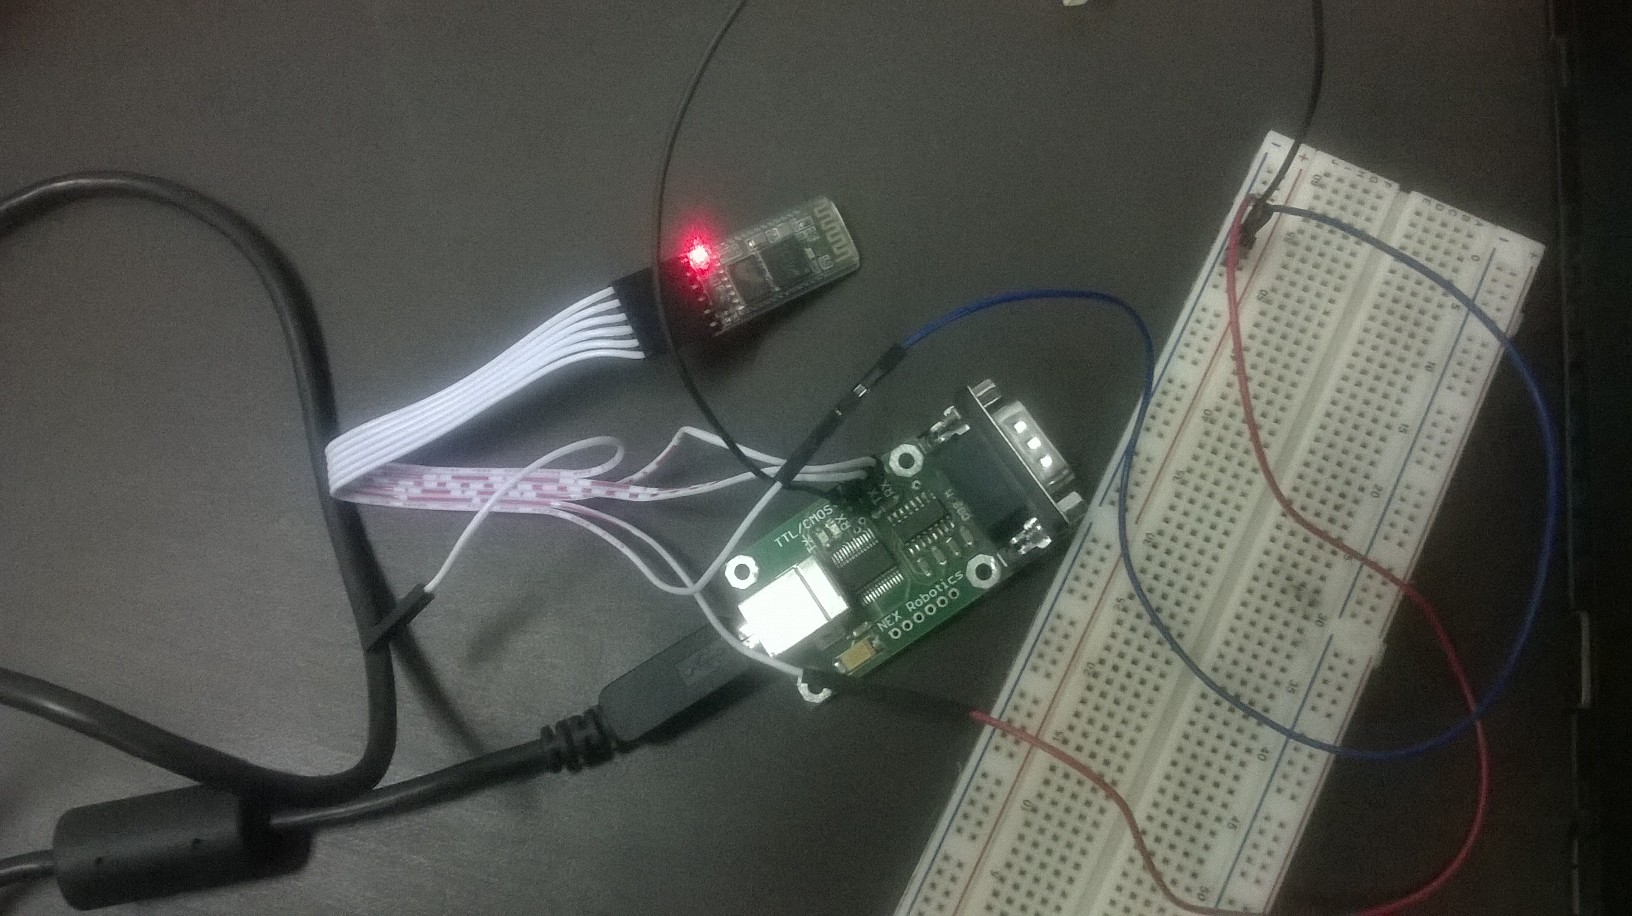
\includegraphics[width=15cm, height=8cm]{BT_Configure}
\end{center}

	\item \textbf{{\large Various AT commands given:}}


\begin{enumerate}
	\item \textbf{AT}


This command is to test the operation. If Response is `OK' then it is working properly.
\\
	\item \textbf{AT+NAME}


This command responds the name of the bluetooth module. Initially the name was ‘Linvor’. We can change the name of the bluetooth module by the command,
AT+NAME=EEG. This command changed the name of bluetooth module with response ‘OK’. To confirm the name, now again give command ‘AT+NAME’.
\\
	\item \textbf{AT+PSWD}

This command responds with its initial password set (1234 ---> Default password).  We have to change the pass code of bluetooth module according to the pass code of the Neurosky EEG sensor as we have to bind it with it. The default password of EEG sensor is ‘0000’. Set the password using command ‘AT+PSWD=0000’. Verify the same with ‘AT+PSWD’.\\


	\item \textbf{AT+CMODE=$<$paratemer$>$}


0----connect the module to the specified Bluetooth address. (Bluetooth address can be specified by the binding command)\\
1----connect the module to any address (The specifying address has no effect for this mode.)\\
2----Slave-Loop\\
Default connection mode: 0\\
We have to connect the bluetooth module only to Neurosky sensor so we give AT command ‘AT+CMODE=0’. To connect mobile or PC/laptop to the bluetooth module we have to change this parameter to 1.
\\

	\item \textbf{AT+UART=$<$param1$>$,$<$param2$>$,$<$param3$>$}


Param1: baud rate( bits/s). The value (Decimal) should be one of the following:\\
4800, 9600, 19200, 38400, 57600, 115200, 23400, 460800, 921600, 1382400\\
Param2:stop bit:\\
0----1 bit\\
1----2 bits\\
Param3: parity bit\\
We have to give the command as ‘AT+UART=9600,0,0’ as the inbuilt baud rate of the sensor is set to 9600 with 1 stop bit and no parity bit.\\



	\item \textbf{AT+ROLE=$<$parameter$>$}


parameter:

0---- Slave role

1---- Master role

2---- Slave-Loop role

Defaule: 0

We have to set the bluetooth module as a master so wealve to give the command as 'AT+ROLE=1', wherein it responds as `OK'.\\
  

	\item \textbf{AT+BIND=$<$parameter$>$}

We need to bind the bluetooth module to the sensor so that it doesn’t get distracted by other bluetooth devices. So we have to configure and bind it using unique ID number of the sensor. The default bind number is 00:00:00:00:00:00. Mindwave Unique Number is given in datasheet as 20:68:9d:88:c1:d7. So we need to give command as AT+BIND=2068,9d,88c1d7.\\


	\item \textbf{AT+IAC=9E8B33}


This is inquiry access code and is used to seek information about all the bluetooth devices around.\\


	\item \textbf{AT+CLASS=$<$parameter$>$}


Param: device type\\
Bluetooth device type is a 32-bit parameter indicates the device type and what typ can be supported.\\
Default: 0\\ 

	\item \textbf{AT+INQM=$<$Param1$>$,$<$Param2$>$,$<$Param3$>$}
Param1: Inquire access mode\\
0----inquiry mode standard\\
1----inquiry mode rssi\\
Param2: the maximum of Bluetooth devices response\\
Param3:The maximum of limited inquiring time\\
The range of limited time: 1~48\\
( Corresponding time:1.28s~61.44s)\\
Default: 1, 1, 48\\
We should give the command as, AT+INQM=1,9,48.\\

\begin{center}
	\graphicspath{ {images/} }
	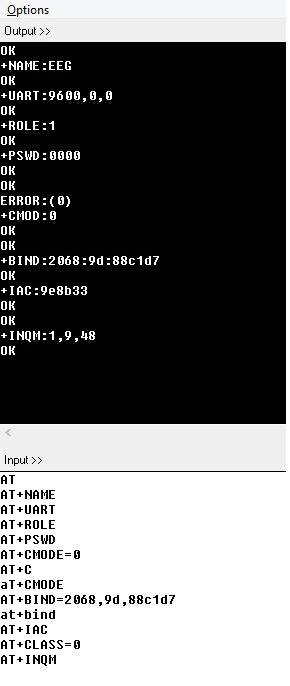
\includegraphics[width=8cm, height=18cm]{BT-AT_Configure}
\end{center}

	\item There are many more AT commands that can be given to change its configuration. But the above given AT commands are sufficient for configuring, binding and interfacing with EEG sensor and Firebird V.\\\\\\\\\\
\end{enumerate}


\end{enumerate}
\end{enumerate}
{\raggedright
\textbf{	References:}
}
\begin{itemize}
	\item •	HC-05 bluetooth module datasheet (uploaded in github link in datasheets folder)
	\item \href{http://upcommons.upc.edu/pfc/bitstream/2099.1/23666/7/Annex3Datasheet\%20mòdul\%20Bluetooth\%20JY-MCU.pdf}{http://upcommons.upc.edu/pfc/bitstream/2099.1/23666/7/Annex3Datasheet\%20mòdul\%20Bluetooth\%20JY-MCU.pdf}
	\item \href{http://www.instructables.com/id/Success-Using-the-JY-MCU-linvor-Bluetooth-Module/step3/The-Correct-Library-Connections/}{http://www.instructables.com/id/Success-Using-the-JY-MCU-linvor-Bluetooth-Module/step3/The-Correct-Library-Connections/}
	\item \href{http://hobbycomponents.com/wireless/64-jy-mcu-bluetooth-wireless-serial-port-module-slave}{http://hobbycomponents.com/wireless/64-jy-mcu-bluetooth-wireless-serial-port-module-slav}
	\item \href{https://github.com/rwaldron/johnny-five/wiki/Getting-Started-with-Johnny-Five-and-JY-MCU-Bluetooth-Serial-Port-Module}{https://github.com/rwaldron/johnny-five/wiki/Getting-Started-with-Johnny-Five-and-JY-MCU-Bluetooth-Serial-Port-Module}
\end{itemize}


\end{document}